We conducted a user study of \evantodo{NUMBER} participants to determine if
there is a statistically significant difference among users in
performing certain tasks on repositories between \textit{Linvis} and
either gitk or the command-line git interface. We were looking for
improvements in accuracy, time performance, and overall enjoyment among
users when performing summarization and intra-tree navigation, as these
are the tasks that merge-trees are design to simplify.

\evan{still need to figure out who our intended user is... ``git user''
  is a bit too broad.}

% TODO: Determine who the intended user is. "generic git user" is kind of broad.
% TODO: Add a note stating that we will refer to the primary branch as being the master branch

\subsubsection{Methodology}
\label{ssub:methodology}

\subsubsection{Commit Selection}
\label{ssub:commit_selection}

We selected two commits for the participant to draw and summarize by
first determining the size of tree in the first and second quartiles. We
found that between Linux 3.1 and 3.16, the size of the trees in the
first quartile only contained a single node, and that the size of the
trees in the second quartile resulted in trees up to seven nodes. The
third quartile contained trees up to 51 nodes, and the fourth quartile
contained one tree of 7217 nodes. It is worth mentioning that the tree
sizes in the fourth quartile increase very quickly, as the next largest
tree only contains 4708 nodes, and the third largest tree contains 2349
commits. We see in figure~\ref{fig:tree_size} how the number of trees
decreases as the size of the tree increases. The results for the other
plots become very noisy, since there is only one occurrence for any tree
with more than 947 commits, and only two occurrences of any trees with
size greater than 336. Due to the noise,
figures~\ref{fig:tree_size_filter},~\ref{fig:merge_count_filter},
and~\ref{fig:percentage_filter} are only on the sizes of trees where
there were at least three occurrences of trees of that size.


\pgfplotstableread[col sep=comma]{data/merge_counts.csv}\mergetable

\begin{figure}
  \centering
  \begin{tikzpicture}
    \begin{axis}[
      ylabel=Occurences,
      xlabel=Total Commits,
      grid=both,
      minor x tick num = 1,
      minor y tick num = 1
      ]
      \addplot[chartblue] table[col sep=comma, x index=1, y index=0]{data/tree_size.csv};
    \end{axis}
  \end{tikzpicture}
  \caption{Frequency of trees of varying sizes}
  \label{fig:tree_size}
\end{figure}


\begin{figure}
  \centering
  \begin{tikzpicture}
    \begin{axis}[
      ylabel=Occurences,
      xlabel=Total Commits,
      grid=both,
      minor x tick num = 1,
      minor y tick num = 1
      ]
      \addplot[chartblue] table[x index=0, y index=1]\mergetable;
    \end{axis}
  \end{tikzpicture}
  \caption{Frequency of trees of varying sizes}
  \label{fig:tree_size_filter}
\end{figure}

\begin{figure}[htpb]
  \centering
  \begin{tikzpicture}
    \begin{axis} [
      ylabel=Merges,
      xlabel=Total Commits,
      minor x tick num = 1,
      minor y tick num = 1,
      grid=both,
      legend pos = north west
      ]
      \addplot[chartred] table[x index=0, y index=5]\mergetable;
      \addlegendentry{Maximum}
      \addplot[chartyellow] table[x index=0, y index=6]\mergetable;
      \addlegendentry{Mean}
      \addplot[chartgreen] table[x index=0, y index=4]\mergetable;
      \addlegendentry{Median}
      \addplot[chartblue] table[x index=0, y index=3]\mergetable;
      \addlegendentry{Minimum}
    \end{axis}
  \end{tikzpicture}
  \caption{Number of merges versus the size of the merge tree}
  \label{fig:merge_count_filter}
\end{figure}

\begin{figure}[htpb]
  \centering
  \begin{tikzpicture}
    \begin{axis} [
      ylabel=Merge Percentage,
      xlabel=Total Commits,
      grid=both
      ]
      \addplot[chartpurple] table[x index=0, y index=7]\mergetable;
    \end{axis}
  \end{tikzpicture}
  \caption{Percentage of commits in a merge-tree that are merge commits}
  \label{fig:percentage_filter}
\end{figure}


As 25\% of the trees consist of a single commit, we selected one tree
consisting of a single commit for the study. 50\% of the trees contained
up to seven nodes, so we selected another tree of size seven.  Of these
trees, we restricted the selection to trees consisting of at least one
merge, not including the merge into the master branch.

From the list of trees consisting of a single node, we selected one at
random using a simple python script and the \verb|random.choice()|
function from python 3.6.1, which returned the merge tree rooted at
\emph{11df5864075f763ec0d1fdecd6a3f0af7d09a553}. As we are not testing
the inter-tree and tree-search capabilities of \emph{Linvis}, we start
the user at the corresponding commit. In this case, there is only a
single option, commit \emph{a3c1239eb59c0a907f8be5587d42e950f44543f8},
shown in Figure~\ref{fig:commit_1}.

\begin{figure}[htpb]
  \centering
  
\includegraphics[width=0.2\linewidth]{figures/commits/1-commit.pdf}
  \caption{The first merge tree used in the user study, a merge tree
    containing a single commit}
  \label{fig:commit_1}
\end{figure}

Using the same merge selection technique, we selected the tree rooted at
\emph{8eb88c80d444fd249edaa7d895666cde79e7b3b8}. To select the starting
commit, we use the python random choice function on the list of commit
hashes contained in this tree. This resulted in the selection of commit
\emph{cdbdd1676a5379f1d5cbd4d476f5e349f445befe}, shown in
Figure~\ref{fig:commit_2}.

\begin{figure}[htpb]
  \centering
  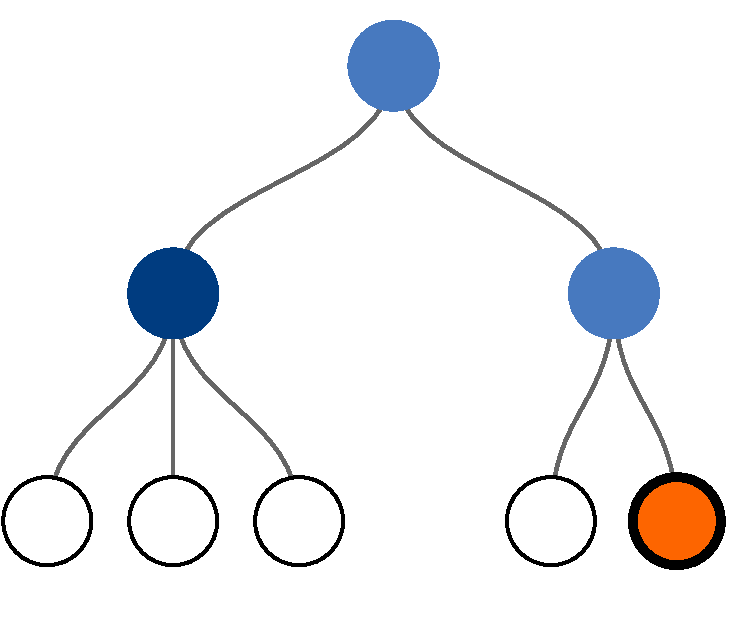
\includegraphics[width=0.5\linewidth]{figures/commits/7-commits.pdf}
  \caption{The second merge tree used in the user study, a merge tree
    containing seven commits}
  \label{fig:commit_2}
\end{figure}

\subsubsection{Questions}
\label{ssub:questions}

We chose questions that were designed to test the two primary goals of
merge trees, compared with the results from gitk or command line git.

\subsubsection{Results}
\label{ssub:results}

\subsubsection{Discussion}
\label{ssub:discussion}

